	\chapter{Sieci neuronowe w muzyce}
	
		Zastosowanie deep learningu do generowania w ostatnim czasie stało się bardzo popularne. Szybki rozwój frameworków takich jak Tensorflow czy Keras pozwala na sprawne budowanie modeli, a wykorzystanie chmur obliczeniowych zwalnia programistę z używania własnego sprzętu bądź też kupowania drogich procesorów GPU. Poniższa grafika obrazuje liczbę publikacji wydanych na przestrzeni ostatnich trzydziestu lat poświęconych generowaniu muzyki z wykorzystaniem deep learningu.
	
	\begin{figure}[H]
		\centering
		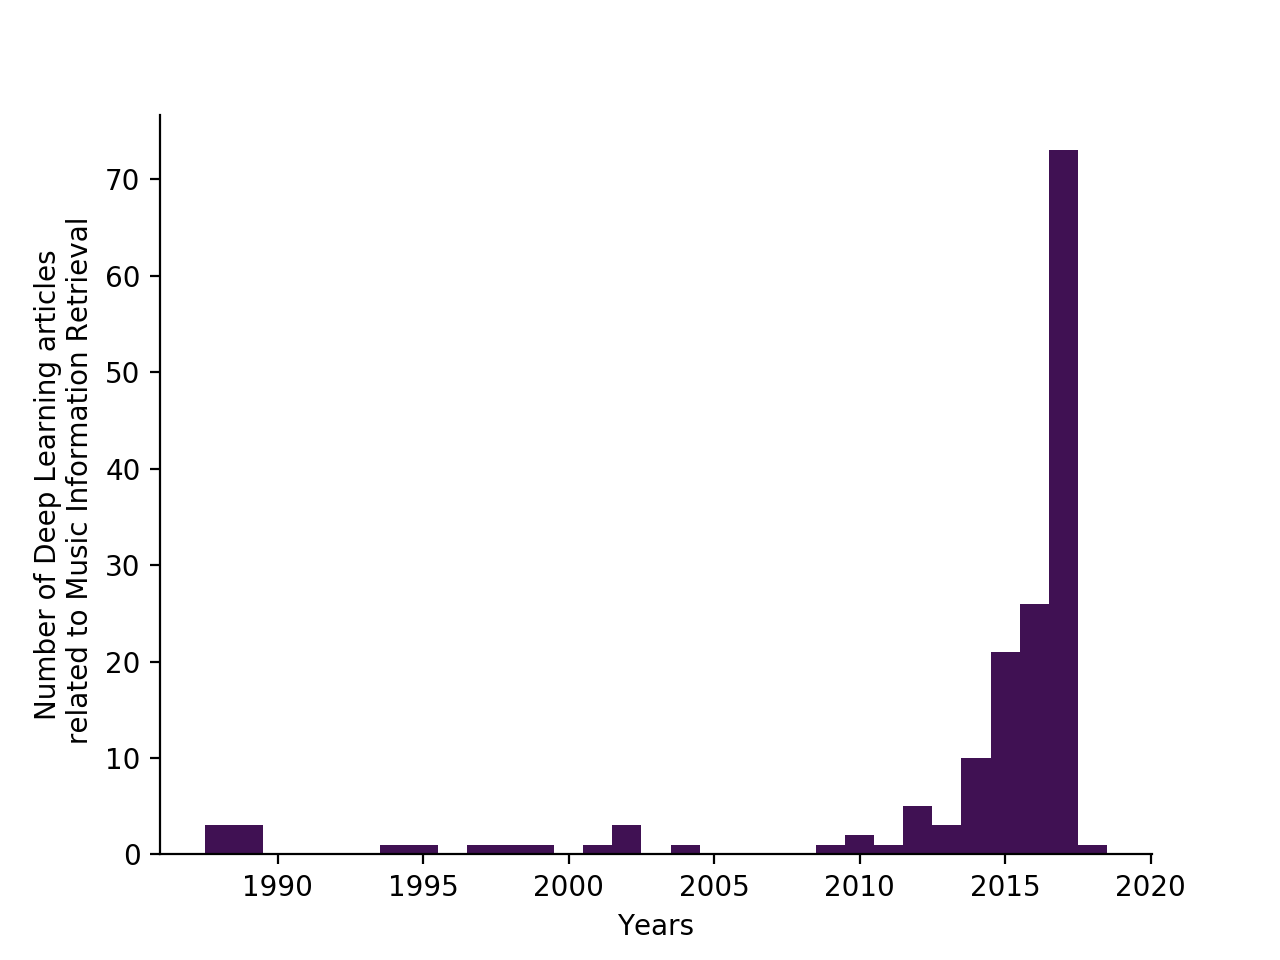
\includegraphics[width=0.7\linewidth]{xxxxxxxxxx}
		\caption{Znaczący wzrost publikacji zanotowany w ostatnich latach \pagenote{\texttt{https://github.com/ybayle/awesome-deep-learning-music/blob/master/dl4m.bib}}}
		\label{fig:xxxxxxxxxx}
	\end{figure}
	
	Obecnie na rynku można wyróżnić sześć dużych projektów związanych z automatycznym generowaniem muzyki. Poniższe podrozdziały będą miały na celu ich charakteryzację. 
	\section{Klasyfikacja narzędzi do tworzenia muzyki}
	
	Programy do generowania muzyki z wykorzystaniem metod deep learningu można poddać klasyfikacji ze względu na ich cechy.	
 Poniższej zostanie przeprowadzona klasyfikacja narzędzi:
 \begin{itemize}
 	\item Magenta$\pagenote{\texttt{https://magenta.tensorflow.org/}}$ - jest to projekt na licencji open source stworzony przez Google. Jak sami autorzy piszą Magenta jest projektem badawczym, który bada rolę uczenia maszynowego w procesie tworzenia sztuki i muzyki. Wiąże się to z ciągłym poszukiwaniem nowych algorytmów deeplearningu. Projekt stanowi również bogate zródło inspiracji dla muzyków i artystów, ponieważ mogą oni wzbogacić swoje procesy za pomocą modeli deep learningu. Przykładem może być tutaj projekt Duet AI$\pagenote{\texttt{https://experiments.withgoogle.com/ai-duet}}$. Magenta powstała na skutek prac inżynierów i badaczy z Google Brain$\pagenote{\texttt{https://ai.google/research/teams/brain}}$. Niestety projekt nie posiada szczegółowej dokumentacji. \text{}\\
 	\centerline{
\includegraphics[width=0.2\linewidth]{magenta-logo}}
 	\item DeepJazz$\pagenote{\texttt{https://deepjazz.io/}}$ - jest efektem pracy Ji-Sung Kima podczas 36 godzinnego hackathonu. \text{}\\
 	\centerline{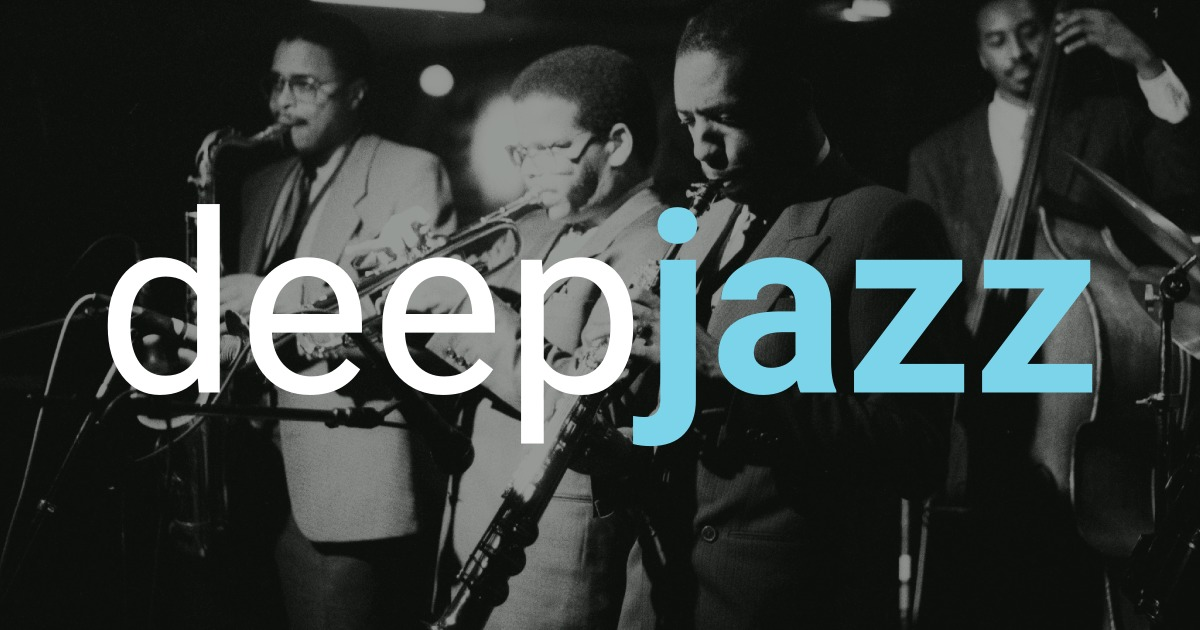
\includegraphics[width=0.2\linewidth]{deep-jazz}}
 	\item BachBot$\pagenote{\texttt{http://bachbot.com/}}$ - projekt badawczy stworzony przez FeynmanaLianga na uniwersytecie w Cambridge \text{}\\
 	\centerline{
\includegraphics[width=0.2\linewidth]{bach-bot}}
 	\item FlowMachines$\pagenote{\texttt{http://www.flow-machines.com/}}$ - projekt badawczy, którego celem jest badanie i rozwijanie systemów sztucznej inteligencji zdolnych do generowania muzyki samodzielnie lub we współpracy z ludźmi. W roku 2017 dzięki FlowMachines udało się wygenerować pełny utwór muzyczny gatunku pop  \text{}\\
 	\centerline{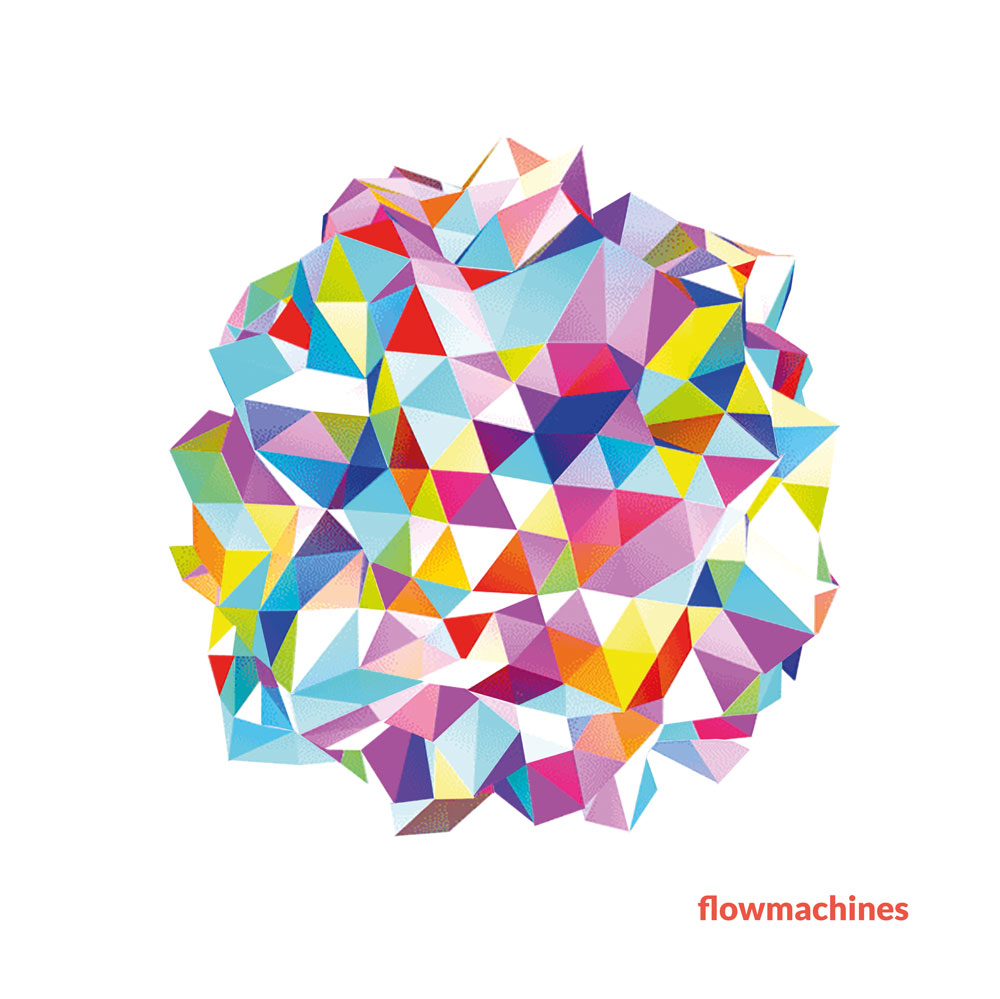
\includegraphics[width=0.2\linewidth]{flow-machines}}
 	\item WaveNet$\pagenote{\texttt{https://deepmind.com/blog/wavenet-generative-model-raw-audio/}}$ - projekt badawczy naukowców z DeepMind. WaveNet bazuje na Konwolucyjnych Sieciach Neuronowych, ta technika bardzo dobrze sprawdza się w klasyfikacji i generowaniu obrazów. Najbardziej obiecującym celem projektu jest poprawa zastosowań zamiany testu na mowę poprzez wygenerowanie bardziej naturalnego przepływu wokalu \text{}\\
 	\centerline{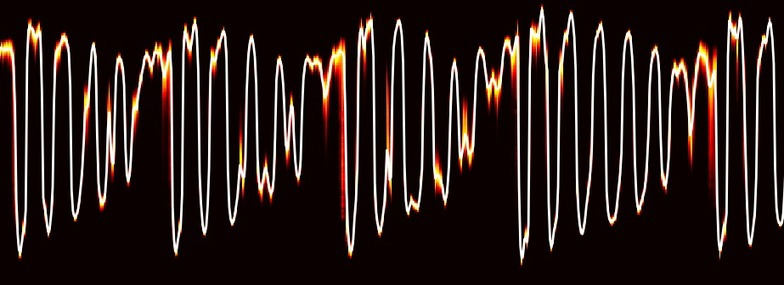
\includegraphics[width=0.2\linewidth]{wave-net}}
 \end{itemize} 

 
 

	\subsection{Klasyfikacja ze względu na dane wejściowe}
	
	Klasyfikacja ze względu na dane wejściowe stanowi ważny punkt w momencie planowania architektury sieci neuronowej. Muzyka jest dostępna w różnych cyfrowych formatach. Począwszy od surowego audio (WAV) do formatów, które pozwalają na zapis semantyki utworu muzycznego - są to formaty takie jak MIDI czy notacja ABC. Aby zdecydować, który format danych jest właściwy należy najpierw postawić pytanie o to w jaki sposób sieć neuronowa będzie pracować i jaka będzie jej architektura. 
	
	Surowy format audio jest bardzo bogatą reprezentacją muzyki, ponieważ potrafi przechować niemal każdy szczegół utworu muzycznego w zależności od formatu i jakości dźwięku. Sygnały audio zawierają barwę instrumentu na podstawie charakterystyki spektrum. Aby wyodrębnić poszczególne nuty z surowego pliku audio konieczne jest zastosowanie transformaty Fouriera. Ze względu na to zastosowanie plików audio jako wejście do sieci neuronowej jest dość złożonym przedsięwzięciem.
	
	W odniesieniu do powyższych projektów można dokonać podziału na dwie kategorie danych wejściowych:
	
	\begin{itemize}
		\item Pliki MIDI
		\item Surowe pliki audio 
	\end{itemize}	
	
	Projektów, które akceptują pliki MIDI jako dane wejściowe jest znacznie więcej niż tych, które akceptują surowe pliki audio. Do tych pierwszych, nazwijmy to formatem tekstowym zaliczają się:
	
		 \textbf{Magenta} - W użyciu biblioteka sprawuje się bardzo dobrze, ponieważ posiada modele wytrenowane na tysiącach plików MIDI. Istnieje możliwość stworzenia własnego modelu na podstawie własnych plików MIDI, które trzeba przekonwertować do protokołu buforowego - NoteSequences stworzonego specjalnie przez Google. Niestety projekt nie posiada szczegółowej dokumentacji. Magenta może generować tylko jeden strumień nut. Nie ma możliwości połączenia kliku modeli np. pianino z perkusją czy gitarą. Trwają prace aby stworzyć model, który będzie wstanie przetwarzać muzykę polifoniczną oraz tworzyć harmonię.
		 
		 \textbf{DeepJazz} - Projekt na wejściu przyjmuje tylko jeden plik MIDI na podstawie, którego odbywa się trening sieci.
		 
		 \textbf{BachBot} - Projekt na wejściu przyjmuje pliki MIDI, dokładnie są to chorały JS Bacha.  
		 
		 \textbf{FlowMachines} - System jest w stanie generować nowe partytury nut w oparciu o styl kompozytora na podstawie bazy około 13000 partytur. 
		 
		 
    	Projekty, które operują na surowych plikach audio to:
	
	
		\textbf{WaveNet} - WaveNet pobiera surowy sygnał audio i syntezuje próbkę wyjściową na podstawie próbki wejściowej. Projekt nie jest oparty o wolny kod źródłowy, ale doczekał się implementacji przez społeczność. Dzięki temu, że sieć używa surowego pliku audio jako wejścia, może generować dowolny instrument. \pagenote{\texttt{https://github.com/ibab/tensorflow-wavenet}} Wykorzystane algorytmy w projekcie są bardzo kosztowne obliczeniowa. Potrzeba kliku minut treningu po to aby wygenerować sekundę dźwięku. Jeden z badaczy pracujący dla Google Sageev Oore z projektu Magenta opisał na swoim blogu jakie wnioski może wyciągnąć kompozytor z wyjścia sieci WaveNet\pagenote{\texttt{https://magenta.tensorflow.org/2016/09/23/learning-music-from-learned-music}}.
		\textbf{GRUV} -  GRUV podobnie jak WaveNet próbuje wykorzystać surowy sygnał audio jako dane wejściowe. Naukowcy z Uniwersytetu Stanforda byli jednymi z pierwszych, którzy pokazali w jaki sposób generować nuty za pomocą sieci LSTM wykorzystując surowe pliki audio jako dane wejściowe.
		 
	\subsection{Klasyfikacja ze względu na architekturę}
	
	\textbf{Magenta} - Aktualnie Magenta implementuje standardową sieć rekurencyjną oraz dwie sieci LSTM. Projekt posiada trzy typy modeli: BasicRNN, LookbackRNN oraz AttentionRNN.
	
	\textbf{DeepJazz} -  Model zawiera dwie warstwy sieci LSTM, które uczą się na podstawie sekwencji nut z plików MIDI.
	
	\textbf{BachBot} - BachBot również wykorzystuje sieci LSTM. 
	 
	\textbf{WaveNet} - WaveNet bazuje na Konwolucyjnych Sieciach Neuronowych, ta technika bardzo dobrze sprawdza się w klasyfikacji i generowaniu obrazów. Najbardziej obiecującym celem projektu jest poprawa zastosowań zamiany testu na mowę poprzez wygenerowanie bardziej naturalnego przepływu części wokalnej.
	
	\textbf{GRUV} -  W przeciwieństwie do WaveNet GRUV wykorzystuje sieci LSTM zamiast CNN. Projekt został opublikowany w 2015 roku\pagenote{\texttt{https://github.com/MattVitelli/GRUV}}. Naukowcy z Uniwersytetu Stanforda byli jednymi z pierwszych, którzy pokazali w jaki sposób generować nuty za pomocą sieci LSTM wykorzystując surowe pliki audio jako dane wejściowe. 
	
	\subsection{Klasyfikacja ze względu na użyte narzędzia}
	Większość projektów korzysta z wysokopoziomowych frameworków do realizacji zadań. Wyróżnić można tutaj trzy duże frameworki: Tensorflow, Keras, Theano. 
	
	 \textbf{Tensorflow} - jest wykorzystywany przez projekt Magenta. Tak samo jak projekt Magenta framework Tensorflow powstał w Google. Tensorflow jest wykorzystywany przez frameworki Keras i Theano - takiego zestawu narzędzi użył Ji-Sung Kim konstruując swój projekt DeepJazz. 
	
	\subsection{Klasyfikacja ze względu na źródła finansowania}
	
	Wielkość projektu często zależy od źródła jego finansowania na wyżej wymienione projekty można podzielić na trzy grupy ze względu na finansowanie:
	
	\begin{itemize}
		\item Unia Europejska - projekt badawczy Flow Machines, został sfinansowany przez Europejską radę ds. Badań Naukowych w ramach 70 programu ramowego UE. Badania zostały zapoczątkowane przez francuskiego naukowca Francoisa Pachet w Sony Computer Science Laboratories (Sony SCL Paris) oraz Uniwersytet Piotra i Marii Curie (UPMC)
		\item Firmy - Google Magenta powstało z wykorzystaniem środków finansowych firmy Google podobnie jak projekt WaveNet
		\item Non profit - projekt DeepJazz został stworzony podczas 36 godzinnego hackathonu.
		\item Granty uniwersyteckie - projekt BachBot został stworzony w murach Uniwersytetu Cambridge, podobnie jak projekt GRUV, który powstał w murach uczelni Stanforda
	\end{itemize}
	
	\section{Własny model sieci}
	
	Celem praktycznym pracy jest przygotowanie własnego modelu sieci neuronowej, który po odpowiednim treningu będzie w stanie wygenerować nuty na podstawie danych treningowych. Model sieci będzie wykorzystał komórki LSTM. Na dane treningowe będą składać się pliki MIDI, w pracy wykorzystano jako jeden z przykładów preludia Fryderyka Chopina. Model został stworzony z wykorzystaniem wysokopoziomowego frameworku Kers, trening odbywał się na maszynie wirtualnej skonfigurowanej w Google Cloud. Projekt składa się z trzech plików:
	
	\begin{itemize}
		\item prepare.py - plik odpowiedzialny za konwersje plików MIDI do formy znakowej
		\item model.py - plik odpowiedzialny za wytrenowanie modelu
		\item generate.py - plik odpowiedzialny za wykorzystanie wytrenowanego modelu
		\item utils.py - plik zawierający pomocnicze funkcje
	\end{itemize}

	Specyfikacja maszyny na której odbywał się trening modelu:
	
	\begin{itemize}
		\item Procesor: Intel(R) Xeon(R) CPU @ 2.20GHz
		\item Karta graficzna: NVIDIA Tesla K80
		\item HDD: 30GB
		\item System operacyjny: Ubuntu 18.04.1 LTS 
		\item Wersja jądra: 4.15.0-1017-gcp
	\end{itemize}

	\subsection{Konfiguracja maszyny w chmurze}
	
	Biorąc pod uwagę potęgę ówczesnych procesorów graficznych bardzo często wykorzystuje się do przetwarzania długich obliczeń. W sieci istnieje szereg usług opartych na chmurze, na których to możemy wypożyczyć sobie konkretną maszynę. Jedyni z popularniejszych usługodawców to:
	
	\begin{itemize}
		\item Google Cloud $\pagenote{\texttt{https://cloud.google.com/}}$
		\item Amazon AWS $\pagenote{\texttt{https://aws.amazon.com/}}$
	\end{itemize}

Na przykładzie użycia Google Cloud opisany zostanie proces tworzenia wirtualnej maszyny oraz jej konfiguracja w celu uruchamiania programów, które mają wykorzystywać procesor GPU. 

Stworzenie nowej instancji wirtualnej maszyny odbywa się z menu \textit{Compute Engine $\rightarrow$ Instancje maszyn wirtualnych}. Następnie należy wybrać przycisk \textit{Utwórz Instancje}

\begin{figure}[H]
	\centering
	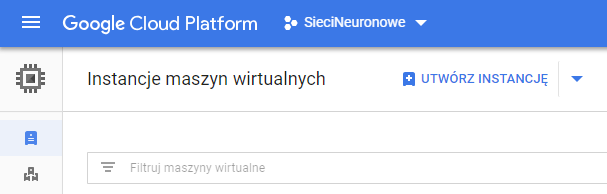
\includegraphics[width=0.7\linewidth]{google_cloud}
	\caption{Tworzenie maszyny wirtualnej}
	\label{fig:googlecloud}
\end{figure}
Kolejny krok do konfiguracja w zależności od potrzeb. Należy pamiętać o tym, że cena maszyny zależy od jej lokalizacji. Maszyna została skonfigurowana w następujący sposób:

\begin{itemize}
	\item Region: us-east1
	\item Liczba procesorów: 4
	\item RAM: 6GB
	\item System operacyjny: Ubuntu 18.04
	\item GPU: Tesla K80
	\item 30GB SSD
	\item Stały adres IP
\end{itemize}	

\begin{figure}[H]
	\centering
	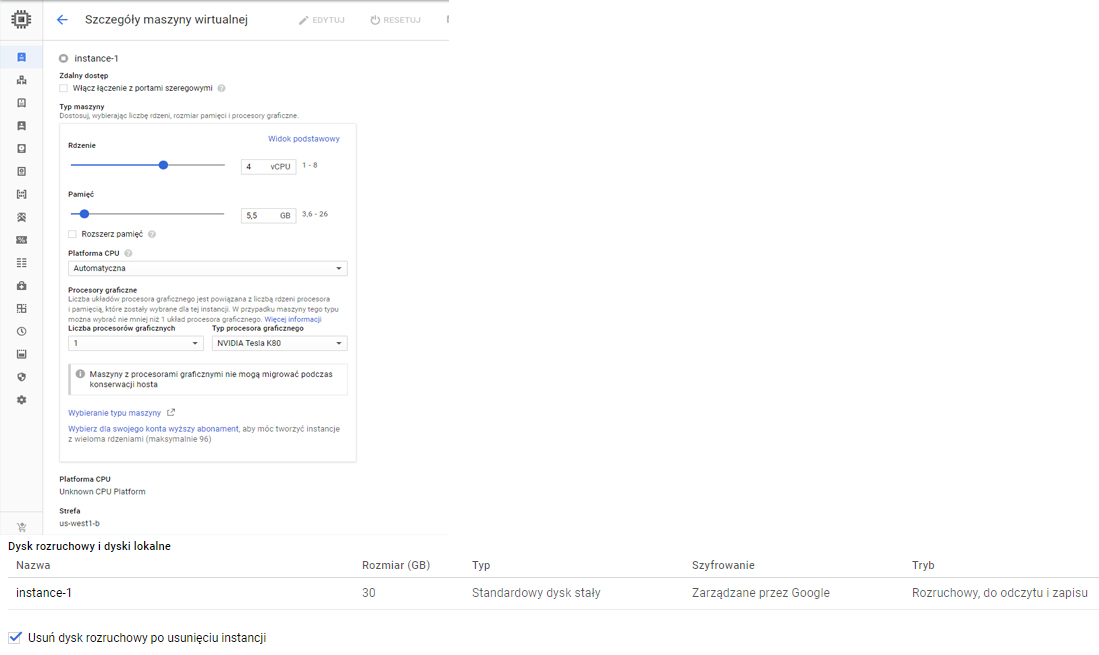
\includegraphics[width=0.7\linewidth]{konfiguracja}
	\caption{Konfiguracja maszyny}
	\label{fig:konfiguracja}
\end{figure}
Po utworzeniu instancji wirtualnej maszyny komunikacja z nią odbywa się za pomocą protokołu SSH z wykorzystaniem kryptografii klucza publicznego i prywatnego. Aby zainstalować biblioteki CUDA należy uruchomić poniższy skrypt, którego zadaniem jest pobranie i instalacja CUDA w wersji 9.2

\begin{lstlisting}[caption={Skrypt instalacyjny sterowników CUDA},captionpos=b]
sudo su
#!/bin/bash

if ! dpkg-query -W cuda; then
sudo apt install gcc-6 g++-6
sudo apt-get install linux-headers-$(uname -r)
sudo apt install nvidia-384
wget -c https://developer.nvidia.com/compute/cuda/9.2/Prod/local_installers/cuda_9.2.88_396.26_linux
chmod +x cuda_9.2.88_396.26_linux.run
./cuda_9.2.88_396.26_linux.run --verbose --silent --toolkit --override
fi
export PATH="$PATH:/usr/local/cuda-9.2/bin"
echo "/usr/local/cuda-9.2/lib64" >> /etc/ld.so.conf
ln -s /usr/bin/gcc-6 /usr/local/cuda-9.2/bin/gcc
ln -s /usr/bin/g++-6 /usr/local/cuda-9.2/bin/g++
\end{lstlisting}

Weryfikacje instalacji można przeprowadzić za pomocą polecenia \textit{nvidia-smi}:
\begin{lstlisting}[caption={Wynik polecenia nvidia-smi},captionpos=b]
+-----------------------------------------------------------------------------+
| NVIDIA-SMI 396.44                 Driver Version: 396.44                    |
|-------------------------------+----------------------+----------------------+
| GPU  Name        Persistence-M| Bus-Id        Disp.A | Volatile Uncorr. ECC |
| Fan  Temp  Perf  Pwr:Usage/Cap|         Memory-Usage | GPU-Util  Compute M. |
|===============================+======================+======================|
|   0  Tesla K80           Off  | 00000000:00:04.0 Off |                    0 |
| N/A   36C    P0    75W / 149W |      0MiB / 11441MiB |    100%      Default |
+-------------------------------+----------------------+----------------------+

+-----------------------------------------------------------------------------+
| Processes:                                                       GPU Memory |
|  GPU       PID   Type   Process name                             Usage      |
|=============================================================================|
|  No running processes found                                                 |
+-----------------------------------------------------------------------------+
\end{lstlisting}
Dodatkowo firma NVIDIA wprowadziła bibliotekę o nazwie cuDNN, której zadaniem jest optymalizacja dla głębokich sieci neuronowych. Wersję cuDNN 8 można pobrać ze strony producenta  \textit{https://developer.nvidia.com/cudnn}. Poniższy skrypt przeprowadzi instalacje pobranego pakietu.
\begin{lstlisting}
tar xzvf cudnn-8.0-linux-x64-v5.1.tgz
sudo cp cuda/lib64/* /usr/local/cuda/lib64/
sudo cp cuda/include/cudnn.h /usr/local/cuda/include/
rm -rf ~/cuda
rm cudnn-8.0-linux-x64-v5.1.tgz
\end{lstlisting}
Środowisko jest już gotowe do uruchamiania programów napisanych z użyciem biblioteki CUDA. Do monitorowania pracy karty graficznej może posłużyć narzędzie \textit{nvtop}$\pagenote{\texttt{https://github.com/Syllo/nvtop}}$.

	
	\section{ Schemat działania modelu}
	
	
	Inspiracją do stworzenia modelu były rozwiązania zastosowane w modelach przeznaczonych do generowania tekstu. W modelowaniu językowym danymi wejściowymi zazwyczaj jest sekwencja słów, a wynik to sekwencja przewidywanych słów. Dana jest długość sekwencji $n$. Sieć ma za zadanie nauczyć się litery, która występuje bezpośrednio po sekwencji długości $n$. Poniżej przykład na podstawie fragmentu Pana Tadeusza.
		
	\lstinputlisting[caption=Pan Tadeusz, style=customc]{pan.txt}
	
	Ustalmy długość sekwencji $n=10$, wówczas ciągi odpowiadające danej literze będą wyglądały następująco:
	
	\lstinputlisting[caption=Sekwencje wszystkich możliwych ciągów, style=customc]{panseq.txt}
	
	W podobny sposób jak język pisany, muzyka działa jako forma ekspresji, w której kombinacje dźwięków mogą wyrażać emocje. Zatem metody, które są wykorzystywane do generowania tekstu z wykorzystaniem deep learningu mogą zostać przełożone na generowanie muzyki. 
	
	Jako dane wejściowe do sieci zostały przygotowane dwa zbiory danych w formacie MIDI:
	\begin{itemize}
		\item 24 Preludia Fryderyka Chopina - 215KB
		\item 21 Sonatin W. A. Mozarta - 668KB
	\end{itemize}
	 Pierwszy etap polega na przygotowaniu danych. Polega to na stworzeniu tablicy, która będzie zawierała wszystkie nuty z wybranego zbioru plików. Początkowy wycinek z tablicy, który powstał przy przetwarzaniu dzieł Fryderyka Chopina: \textit{['C2', 'G3', 'G2', 'C4', 'E3', 'G4', 'E4', 'C4', 'A4', 'A3', 'B1', 'G3', 'G2', 'D4', 'F3', 'G4', 'F4', 'D4', 'A4', 'A3']} odpowiada pierwszemu preludium z Opusu 28. Tablica przechowuje tylko wysokość danej nuty, inne cechy utworu muzycznego nie są wykorzystywane.
	
	\begin{figure}[H]
		\centering
		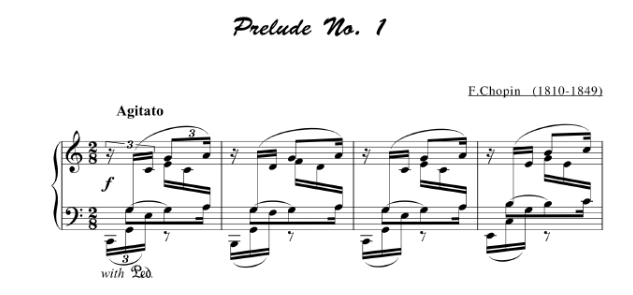
\includegraphics[width=0.7\linewidth]{prelude_no_1}
		\caption{Początkowy fragment preludium}
		\label{fig:preludeno1}
	\end{figure}	
	Liczba wszystkich unikalnych nut zależy od wybranego zbioru danych. Kolejnym krokiem jest stworzenie słownika, który przyporządkuje daną nutę lub akord kolejnej liczbie naturalnej. Rozmiar słownika powinien wynosić tyle ile jest unikalnych nut i akordów.
	
	Następnie w trzecim kroku należy stworzyć sekwencje wejściowe dla sieci i ich odpowiednich wyjść. Wyjście dla każdej sekwencji wejściowej będzie pierwszą nutą lub akordem, która pojawia się po sekwencji nut w sekwencji wejściowej na naszej liście nut.
	
	\lstinputlisting[caption=Sekwencje wejściowe i odpowiadające im nuty, style=customc]{noteseq.txt}
	
	Do przewidywania prawdopodobieństwa użycie średniego błędu kwadratowego (RMSE) jako funkcji kosztu nie jest właściwe. Jako funkcja kosztu zostanie wykorzystana funkcja entropii krzyżowej kategorycznej. 
	
	\begin{equation}
	L_{i} = - \sum_{j}t_{i,j} log(p_{i,j})
	\end{equation}
	
	Funkcja ta jest odpowiednia do przewidywania wartości ze zbioru wieloklasowego. Jest również domyślnym wyborem przy połączeniu z funkcją aktywacji softmax. Ostatnim krokiem w przygotowaniu modelu jest normalizacja danych wejściowych oraz zapewnienie one-hot encoding dla danych wyjściowych. Kodowanie wyjścia polega na tym, że na pozycji określającej daną klasę stoi jedynka, a na pozostałych zą zera. Poniższy przykład ilustruje kodowanie cyfr. 
	
	\begin{itemize}
		\item cyfra '0' zostanie zakodowana jako [1,0,0,0,0,0,0,0]
		\item cyfra '1' zostanie zakodowana jako [0,1,0,0,0,0,0,0]
		\item cyfra '9' zostanie zakodowana jako [0,0,0,0,0,0,0,1]
	\end{itemize}
	
	Kodowanie zostanie wykorzystane do zakodowania etykiet poszczególnych nut, które znajdują się we wcześniej stworzonym słowniku. 
	
	\subsection{Architektura modelu}
	
	Model sieci neuronowej został przygotowany w oparciu o wysokopoziomowy framework Keras. Domyślna architektura sieci składa się z pięciu warstw:
	
	\begin{itemize}
		\item LSTM z 128 wejściami
		\item Dropout
		\item LSTM z 128 wejściami
		\item Dropout
		\item Warstwa wyjścia składająca się z N neuronów, gdzie N odpowiada liczbie unikalnych nut w wybranym zbiorze danych
	\end{itemize}

	Do modelu zostały dobrane następujące domyślne parametry:
	
	\begin{itemize}
		\item Funkcja straty: entropia krzyżowa
		\item Optymalizator: Adam
		\item Stała uczenia: 0.001
		\item Podział na zbiór testowy i walidacyjny: 0.2
	\end{itemize}	
	
	Wykorzystując uczenie nadzorowane, model sieci neuronowej ma za zadanie wytrenować model. W modelu używane są dwa zestawy danych jako dane wejściowe. Można je zdefiniować jako: sekwencje nut długości $n$ - $X$ oraz klasa predyktorów czyli pojedyncze nuty, które występują bezpośrednio po danej sekwencji - $y$. Dane wejściowe zostały podzielone również na zestawy szkoleniowe i walidacyjne aby móc sprawdzić poprawność działania modelu. 
		
	\section{Szczegółowy opis programu}
	
	Pierwszym etapem przy pracy z programem jest przygotowanie danych wejściowych do sieci. Ze względu na to, że format MIDI nie zawiera bezpośrednio danych tekstowych trzeba je wydobyć. Do konwersji plików MIDI na dane tekstowe wykorzystana została biblioteka music21. Jeżeli w utworze muzycznym występują akordy to są one rozbijane na poszczególne nuty składowe. Po konwersji wszystkich plików dane w postaci binarnej są zapisywane do pliku aby przy ponownym uruchomieniu programu uniknąć ponownej konwersji plików. Domyślna nazwa katalogu, w którym są przechowywane pliki MIDI to \textit{midi}. Dodatkowo za pomocą programu można dokonać transpozycji wszystkich plików midi do wybranej tonacji. Pomoc do pliku można wyświetlić za pomocą przełącznika -h. 
	
	\begin{lstlisting}[caption={Pomoc do programu prepare.py},captionpos=b]
	usage: prepare.py [-h] [--midi_dir MIDI_DIR] [--out_file OUT_FILE]
	[--transpose TRANSPOSE]

	optional arguments:
	-h, --help            show this help message and exit
	--midi_dir MIDI_DIR   MIDI files directory containing. mid files (default:
	midi/)
	--out_file OUT_FILE   Path to file containing done parse MIDI files
	(default: data/notes)
	--transpose TRANSPOSE
	Key to transpose all MIDI files (default: None)
	
	\end{lstlisting}
	
	Dane w postaci binarnej są zapisywane do pliku z wykorzystaniem biblioteki \textit{pickle}. Dane domyślnie zapisywane są w katalogu \textit{data}.
	
	Po wstępnym przygotowaniu danych należy użyć pliku train.py. Plik ten, zawiera domyślny model sieci neuronowej oraz szereg parametrów, które można zmieniać za pomocą odpowiednich przełączników. Program jest odpowiedzialny za przygotowanie danych do sieci oraz za trening modelu. Aby użyć modelu, plik z danymi może być wcześniej przygotowany przez program \textit{prepare.py}. Jeżeli wcześniej przygotowany plik z danymi nie istnieje, można użyć domyślnego lub za pomocą opcji --midi\_dir przygotować własny. Pomoc do pliku można wyświetlić za pomocą przełącznika -h.	
	
	\begin{lstlisting}[caption={Pomoc do programu train.py},captionpos=b]
	$ python3 train.py -h
	usage: train.py [-h] [--midi_dir MIDI_DIR] [--data_file DATA_FILE]
	[--results_dir RESULTS_DIR] [--lstm_size LSTM_SIZE]
	[--layers LAYERS] [--learning_rate LEARNING_RATE]
	[--sequence_size SEQUENCE_SIZE] [--batch_size BATCH_SIZE]
	[--dropout DROPOUT]
	[--optimizer {sgd,rmsprop,adagrad,adadelta,adam,adamax,nadam}]
	[--activation {softmax,sigmoid,linear,tanh,elu,selu,softplus,softsign,relu}]
	
	optional arguments:
	-h, --help            show this help message and exit
	--midi_dir MIDI_DIR   MIDI files direcotry containing .mid files to use for
	training neural network (default: midi)
	--data_file DATA_FILE
	Path to file containing done parse MIDI files
	(default: data/notes-preludia)
	--results_dir RESULTS_DIR
	Directory to store model in JSON format, logs for
	tensorboard and weights (default: results)
	--lstm_size LSTM_SIZE
	Size of LSTM layer (default: 128)
	--layers LAYERS       Number of layers in the neural network (default: 2)
	--learning_rate LEARNING_RATE
	Learning rate (default: 0.0001)
	--sequence_size SEQUENCE_SIZE
	Sequence size for notes (default: 100)
	--batch_size BATCH_SIZE
	Batch size (default: 128)
	--dropout DROPOUT     Dropout percentage value. One of regularization method
	(default: 0.3)
	--optimizer {sgd,rmsprop,adagrad,adadelta,adam,adamax,nadam}
	Optimization algorithm to use (default: rmsprop)
	--activation {softmax,sigmoid,linear,tanh,elu,selu,softplus,softsign,relu}
	Activation function to use (default: softmax)
	
	\end{lstlisting}
	Każdorazowe uruchomienie programu \textit{train.py} powoduje utworzenie na katalogu \textit{results} podkatalogu, który zawiera:
	
	\begin{itemize}
		\item bieżący model sieci neuronowej w formacie JSON
		\item wagi 
		\item logi przeznaczone do wyświetlenia w \textit{tensorboard}\pagenote{\texttt{https://www.tensorflow.org/guide/summaries\_and\_tensorboard}}
	\end{itemize}
		
	Po wczytaniu pliku z danymi program musi odpowiednio zmapować dane, ponieważ sieć neuronowa potrzebuje danych numerycznych, a w tym momencie są dostępne dane w formie łańcuchów znaków. Po konwersji danych na dane liczbowe następuje przygotowanie sekwencji wejściowych i odpowiednich wyjść dla danej sekwencji. Jest tutaj wykorzystywany parametr o nazwie \textit{--sequence\_size}, który informuje o długości sekwencji, domyślnie ma wartość 100, którą można zmodyfikować.
		
	Następnie dane są normalizowane oraz przygotowywane jako wejście do sieci z wykorzystaniem techniki one-hot-encoding. Podczas treningu modelu wagi są co jakiś czas zapisywane do plików .hdf5 po to aby po zakończeniu treningu można było wybrać odpowiedni zestaw wag biorąc pod uwagę błąd oraz dopasowanie modelu. Jest to też pewnego rodzaju zabezpieczenie przed nieoczekiwanym zatrzymaniu modelu. 
	
	Proces uczenia sieci można obserwować w czasie rzeczywistym wydając polecenie:
	
	\begin{lstlisting}[caption={Wykorzystanie tensorboard do wizualizacji wyników},captionpos=b]
		tensorboard --logdir resuts/
	\end{lstlisting}
	
	Po wytrenowaniu modelu można podjąć próbę wygenerowania nut. Do tego celu jest potrzebny ostatni plik generate.py. Uruchomienie pliku wymaga podania dwóch argumentów. Pierwszy z argumentów wskazuje na wybrany plik z wagami. Drugi musi wskazywać na wcześniej stworzony plik z nutami, który był wykorzystywany do trenowania sieci.
	
	\begin{lstlisting}
	python3 generate.py --weights weights.hdf5 --notesfile filepath
	\end{lstlisting}	
	
	Program domyślnie podejmie próbę wygenerowania 1000 nut, można tę długość zmienić za pomocą opcjonalnego parametru --len:
	
	\begin{lstlisting}
	python3 generate.py --weights weights.hdf5 --notesfile filepath --len 500
	\end{lstlisting}	
	
	Aby wykorzystać sieć neuronową do generowania muzyki należy wykorzystać dokładnie tą samą sieć, która była użyta do treningu. Jednak sieć nie będzie ponownie szkolona. Zostanie wypełniona tymi samymi danymi oraz jako wagi zostaną wykorzystane wagi, które powstały na skutek treningu sieci w poprzednim kroku. Po załadowaniu wag do modelu można go użyć do generowania nut. Jako punkt startowy wybierany jest losowy indeks z danych wejściowych. Pozwala to na kliku krotne generowanie nut na tych samych danych wagowych z różnymi wynikami przy każdej próbie. Ze względu na to, że sieć posiada tylko dane numeryczne konieczne jest zdekodowanie każdej wartości liczbowej na odpowiednią nutę. Do każdej wygenerowanej nuty, która ma być wygenerowana musi zostać przypisana odpowiednia sekwencja. Pierwsza sekwencja jest wybierana losowo. Z każdej kolejnej sekwencji, która jest używana jako wejścia usuwana jest pierwsza nuta i wstawiany jest wynik z poprzedniej iteracji. Do określenia najbardziej prawdopodobnej nuty na podstawie danych wejściowych z sieci wybierany jest indeks, który posiada największe prawdopodobieństwo wystąpienia po danej sekwencji. Cały proces jest powtarzany, a dane są gromadzone w tablicy. 	
	
	\subsection{Użyte narzędzia}
	
	W projekcie użyto następne wersje narzędzi:
	
	\begin{itemize}
		\item \textbf{Python 3.6 } - język programowania powszechnie używany w uczeniu maszynowym
		\item \textbf{Keras 2.2.2 } - wysokopoziomowa biblioteka, która umożliwia tworzenie sztucznych sieci neuronowych. Biblioteka używa TensorFlow lub Theano. 
		\item \textbf{Tensorflow GPU 1.10.0 }- biblioteka stworzona przez zespół Google Brain, która ma zastosowanie w uczeniu maszynowym oraz głębokich sieciach neuronowych. Obliczenia mogą być wykonywane na procesorze CPU lub GPU.
		\item \textbf{Tensorboard} - narzędzie, które umożliwia wizualizowanie sieci neuronowej podczas nauki. Pozwala to na wcześniejsze ocenienie czy proces uczenia będzie pomyślny.
		\item \textbf{music21} - rozbudowana biblioteka służąca do pracy z muzyką. Za jej pomocą można analizować pliki MIDI i je tworzyć. 
		\item \textbf{sklearn} - biblioteka, która ma zastosowanie w uczeniu maszynowym. 
		\item \textbf{numpy} - biblioteka służąca do wykonywania obliczeń matematycznych
		\item \textbf{matplotlib} - biblioteka służąca do rysowania wykresów
		\item \textbf{CUDA 9.0.176} - \textit{Compute Unfied Device Architecture} jest to opracowana przez firmę NVIDIA architektura procesorów GPU, która umożliwia wykorzystanie procesorów GPU do rozwiązywania problemów numerycznych
	\end{itemize}

	\subsection{Wyniki}
	
	W zależności od układu i liczby warstw wyniki działania sieci neuronowej są różne. Częstym problemem w otrzymanych wynikach było to, że sieć została przeuczona co wynikało z tego, że krzywa zbioru walidacyjnego znacznie odbiegała od krzywiej zbioru testowego. Nie przeszkodziło to jednak w generowaniu utworu. Chociaż można usłyszeć, że wygenerowany utwór zawiera frazy, które zostały wyciągnięte bezpośrednio ze danych uczących się. Poniżej przedstawiono kilka lepszych rezultatów z wielu podejmowanych prób w różnych konfiguracjach sieci. 
	
	\begin{figure}[H]
		\centering
		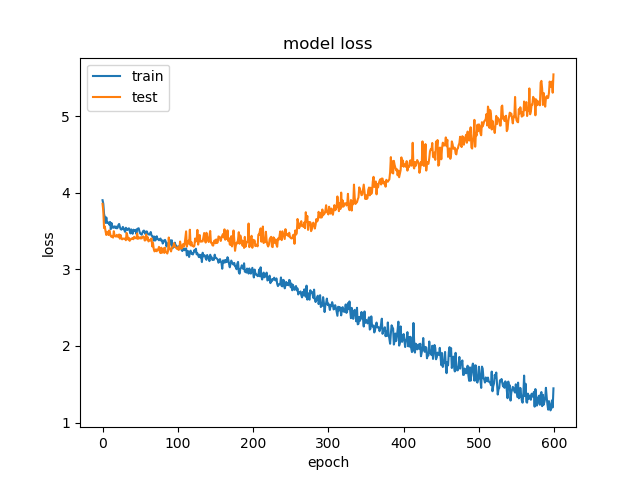
\includegraphics[width=0.5\linewidth]{uWq2G}
		\caption{Przeuczenie sieci}
		\label{fig:uwq2g}
	\end{figure}
	Dzięki temu, że podczas treningu model zapisuje wagi co jakiś czas można było wykorzystać wagi z epoki 200 do wygenerowania nowych nut. W wyniku powstał plik MIDI, który muzycznie może przypominać styl preludiów. Co ważne, wygenerowany utwór nie jest chaosem losowo wybranych nut co może świadczyć o potencjale sztucznych sieci neuronowych na polu generowania muzyki. Poniżej fragment wygenerowanego utworu. 
	\begin{figure}[H]
		\centering
		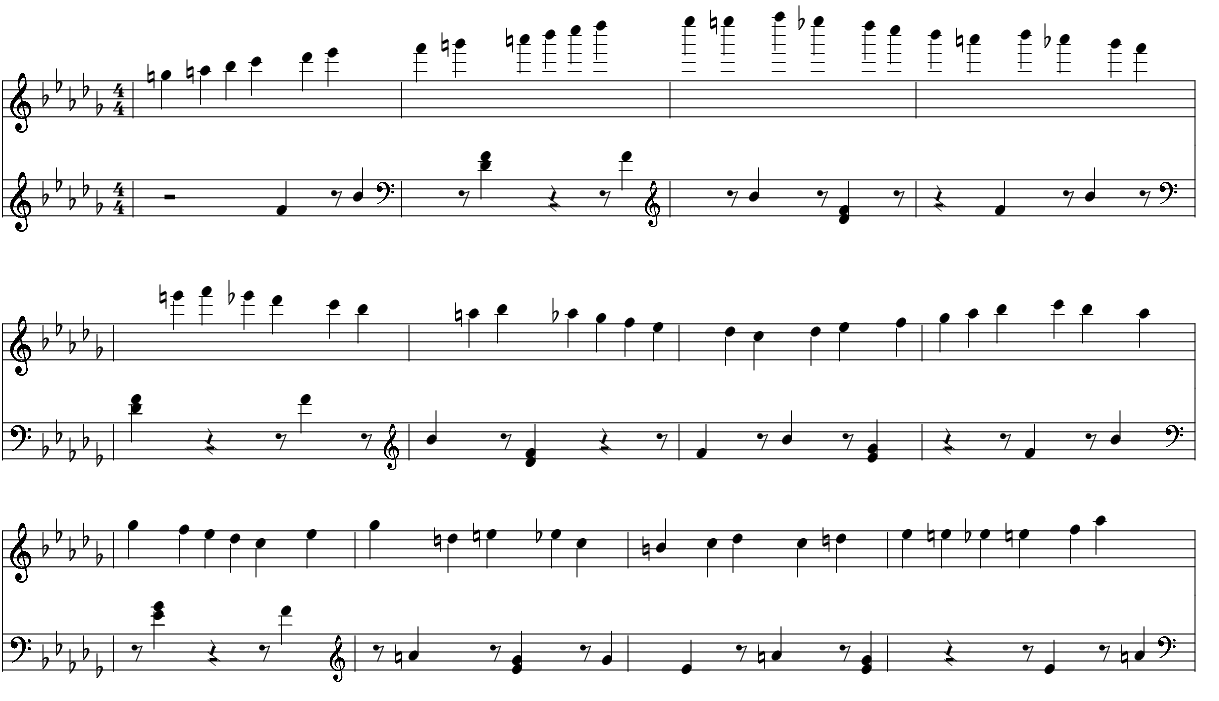
\includegraphics[width=0.7\linewidth]{wygenerowane_preludium}
		\caption{Początkowy fragment wygenerowanego utworu}
		\label{fig:wygenerowanepreludium}
	\end{figure}

	Inny wynik został uzyskany wykorzystując model, który składał się z dwóch warstw LSTM. 
	\begin{figure}[H]
		\centering
		\includegraphics[width=0.5\linewidth]{"2 przyklad/history_loss"}
		\caption{Wykres błędu}
		\label{fig:historyloss}
	\end{figure}

	Wykres niestety też nie jest zadowalający, ale nie przeszkadza to przy wygenerowaniu utworu. Poniżej wykres przedstawiający dopasowanie modelu.
	\begin{figure}[H]
		\centering
		\includegraphics[width=0.7\linewidth]{"2 przyklad/acc_history"}
		\caption{Dopasowanie modelu}
		\label{fig:acchistory}
	\end{figure}

	\begin{figure}[H]
		\centering
		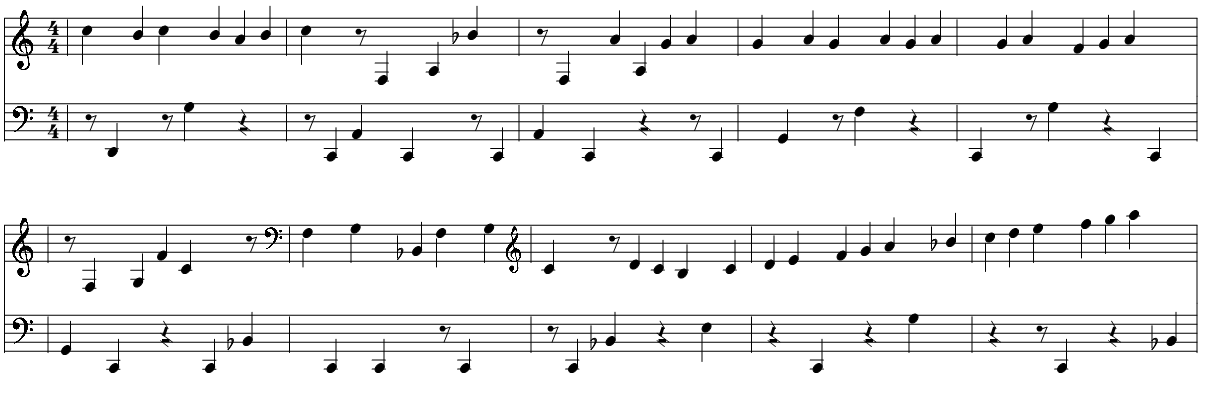
\includegraphics[width=0.7\linewidth]{2przyklad}
		\caption{Fragment utworu, który został wygenerowany z użyciem dwóch warstw LSTM}
		\label{fig:2przyklad}
	\end{figure}	
	
	\subsection{Wnioski}	
	
	Wykorzystanie sieci neuronowych sprawdza się w przypadku generowania muzyki. Sieci są w stanie przetworzyć duże zbiory danych. Problem pojawia się w przypadku uczenia modelu, ponieważ ten przeucza się. Rozwiązanie tego problemu może leżeć w nieprawidłowym przygotowaniu danych wejściowych. Należałoby oddzielnie zająć się harmonią (lewą ręką) i melodią (prawą ręką)$\pagenote{Yoav Zimmerman, \textit{A Dual Classification Approach to Music Language Modeling}, 2016}$ dodatkowo takie elementy jak tempo czy dynamika mogłyby być rozpoznawane przez sieć. Wymaga to dodatkowych eksperymentów na polu rekurencyjnych sieci neuronowych. Niestety nie ma jednoznacznego przepisu co do ilości warstw, algorytmu optymalizacji czy funkcji aktywacji należy na zasadzie prób i błędów wybrać odpowiednią konfiguracje. Możliwe, że zastosowanie komórki podobnej do LSTM - GRU$\pagenote{\texttt{https://arxiv.org/pdf/1702.07787.pdf}}$ \textit{(Gated recurrent unit)}, które są lżejsze obliczeniowo wpłynęłoby na otrzymane wyniki. W ostatnim czasie dużą popularność zyskały sieci typu \textit{GAN} (Generative Adversarial Nets) $\pagenote{\texttt{https://arxiv.org/pdf/1406.2661.pdf}}$. \textit{Generative Adverial Nets }są również wykorzystywane na polu generowania muzyki$\pagenote{\texttt{https://salu133445.github.io/musegan/}}$.
		
	\chapter*{Zakończenie}
	Współczesne techniki informatyczne w połączeniu z matematyką dają szerokie pole manewru w dziedzinie generowania muzyki bądź w dziedzinie komponowania muzyki. Niewątpliwie ważną cechą jest prawidłowe przygotowania danych. Sieci neuronowe w kontekście muzyki mają duże znaczenie, a łańcuchy Markowa i gramatyki mogą pośredniczyć w przygotowaniu końcowego modelu. W ostatnim czasie powstały sieci służące typowo do zadań generatywnych \textit{Generative adversarial networks}, które zostały przedstawione przez Iana Goodfelow w 2014. Rozległość i ciągły rozwój metod sztucznej inteligencji pozwala na szeroką gamę możliwości empirycznego eksperymentowania w dziedzinie generowania muzyki czy też wspomagania kompozytorów w tworzeniu muzyki. 